\pgfplotsset{compat=1.15}
\setlength{\fboxsep}{0pt}

\begin{tikzpicture}
  \draw
  (0, 8) node[anchor=east, scale=0.8]{Input} to[short, o-]
  ++(1, 0) node[anchor=west,inner sep=0](extract){
    \fbox{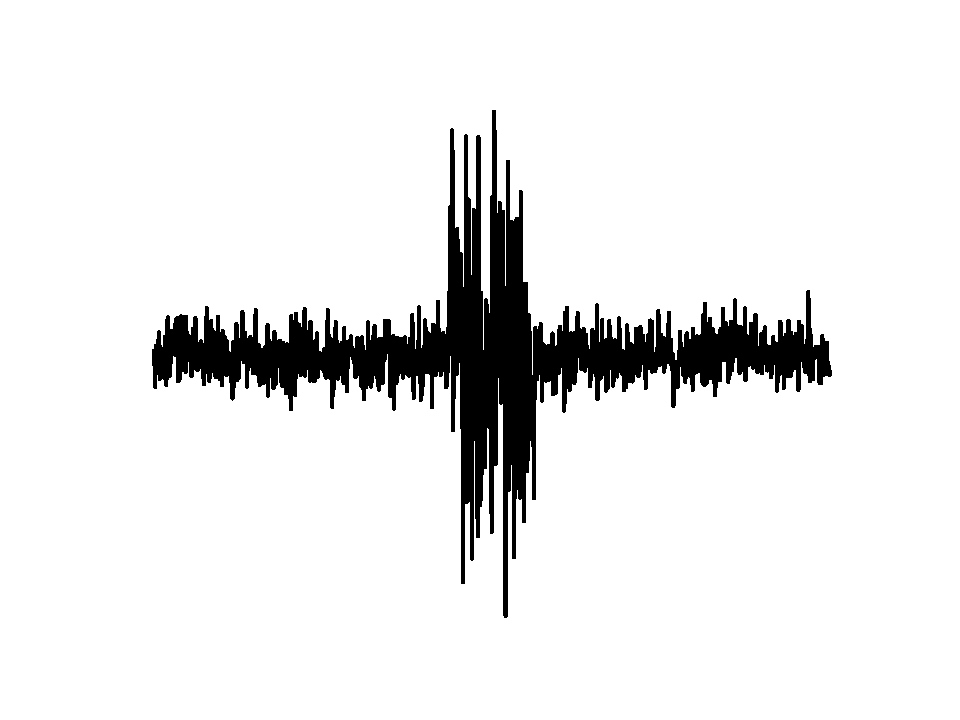
\includegraphics[width=2cm]{diagrams/xcorr_tagger_extract.pdf}}
  }
  (extract.east) to[short]
  ++(1, 0) coordinate(insplit) to[short]
  ++(0, 1.5) to[short]
  ++(0.5, 0) to[short, -*]
  ++(0, 0.25) coordinate(xcorrmerge) to[short]
  ++(1, 0) node[anchor=west,inner sep=0](xcorrdiag){
    \fbox{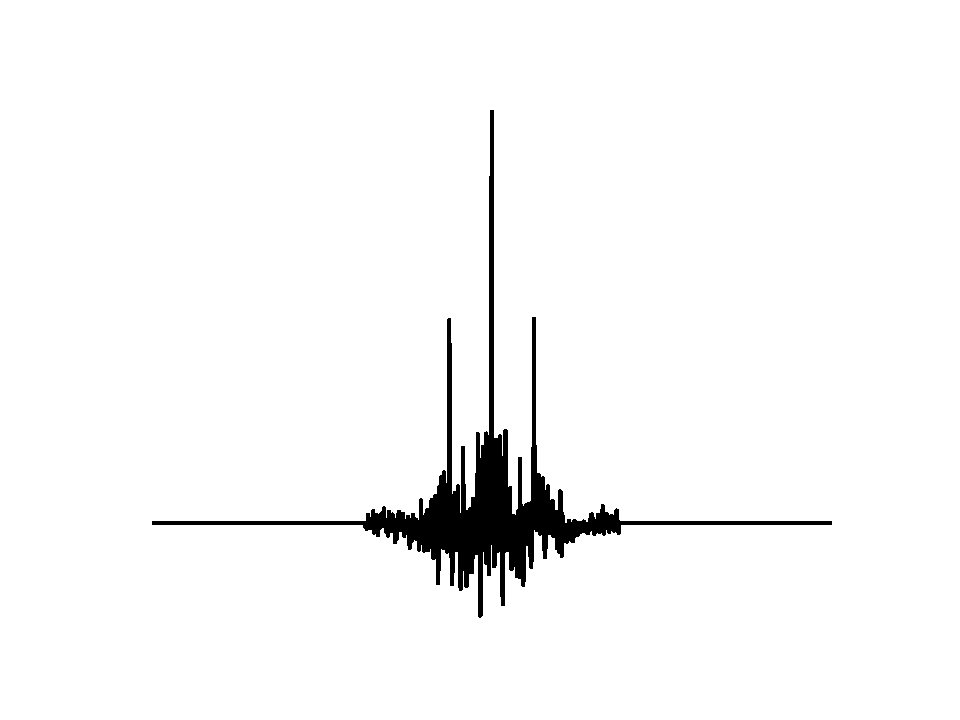
\includegraphics[width=2cm]{diagrams/xcorr_tagger_find_max.pdf}}
  };

  \draw
  (xcorrmerge) to[short]
  ++(0, 0.25) to[short]
  ++(-1.5, 0) node[anchor=east,inner sep=0](preamble){
    \fbox{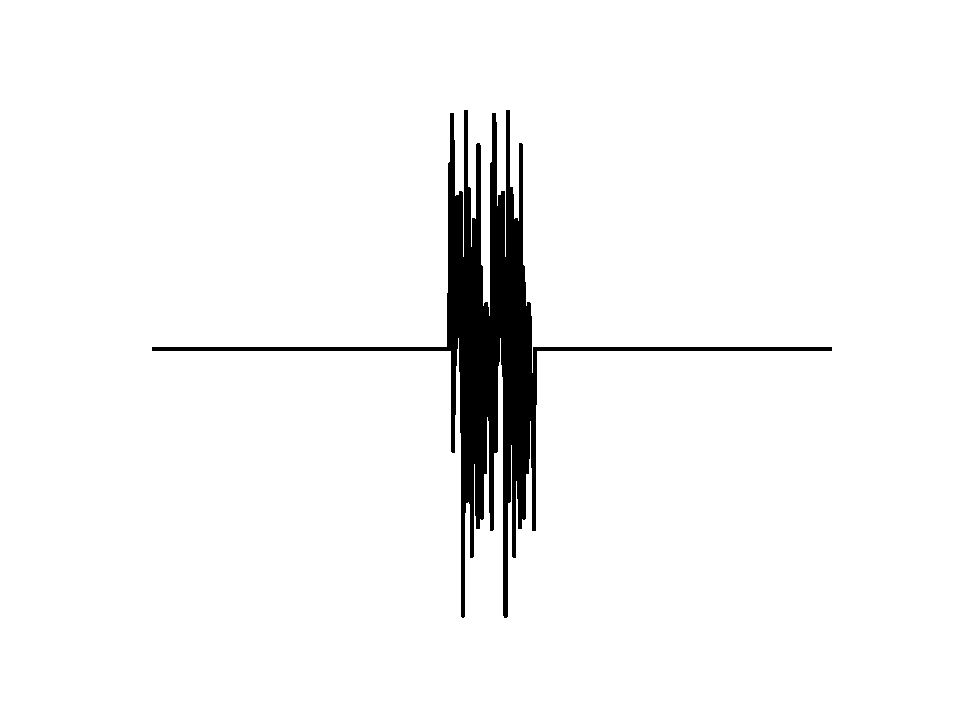
\includegraphics[width=2cm]{diagrams/xcorr_tagger_sync_padded.pdf}}
  }
  (preamble.north)
  ++(0, 0.01) node[anchor=south, scale=0.6]{Stored preamble};

  \draw
  (xcorrmerge)
  ++(0, 0.3)
  node[anchor=south, scale=0.6, align=center]{Cross-\\correlation};

  \draw
  (insplit) to[short]
  ++(0, -1.25) to[short, -*]
  ++(0.5, 0) coordinate(schcoxpoint) to[short]
  ++(1, 0) node[anchor=west,inner sep=0](schcox){
    \fbox{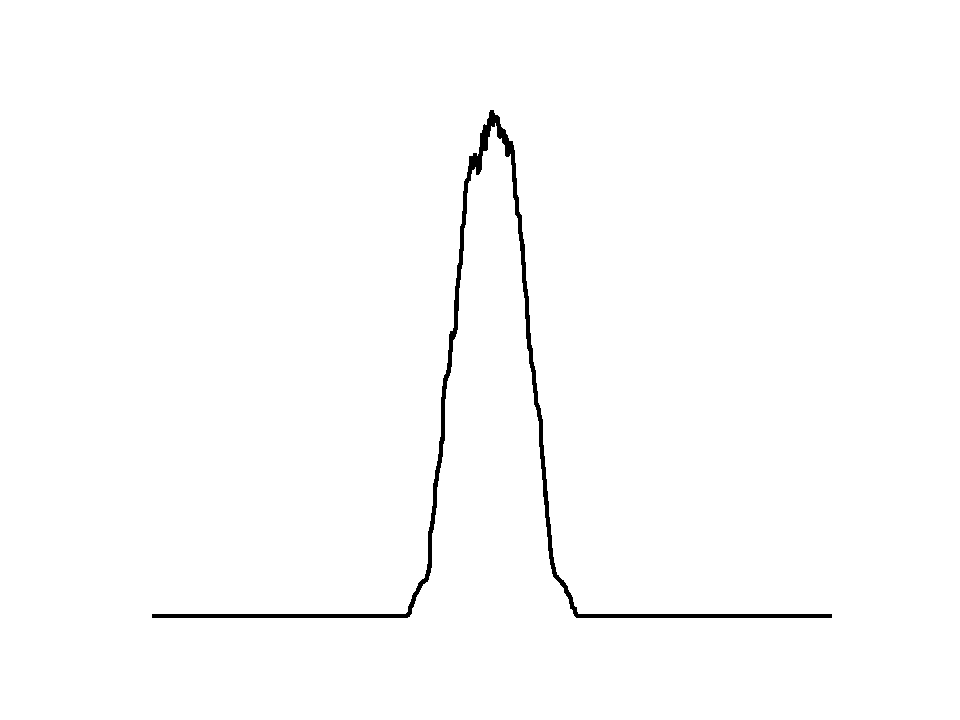
\includegraphics[width=2cm]{diagrams/xcorr_sc.pdf}}
  }
  (schcoxpoint)
  ++(0, -0.1) node[anchor=north, scale=0.6]{Schmidl \& Cox};

  \draw
  (xcorrdiag.east) to[short]
  ++(0.75, 0) to[short]
  ++(0, -1.5) node(out_mul)[mixer, scale=0.5, anchor=north]{}
  (out_mul.south) to[short]
  ++(0, -1.01) to[short]
  (schcox.east);

  \draw
  (out_mul.east) to[short]
  ++(0.75, 0) node[anchor=west,inner sep=0](outdiag){
    \fbox{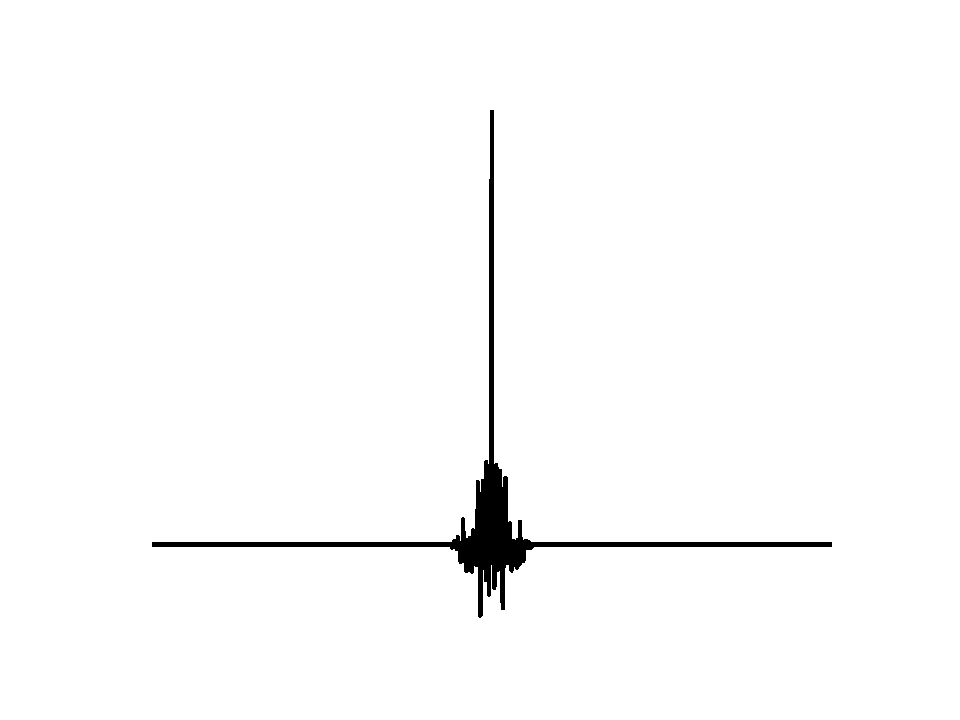
\includegraphics[width=2cm]{diagrams/xcorr_tagger_find_max_masked.pdf}}
  }
  (outdiag.east) to[short, -o]
  ++(0.75, 0) node[anchor=west, scale=0.8]{Output};

  \draw[densely dotted]
  (-1, 6) --
  ++(3.5, 0) --
  ++(6.5, 3.5) --
  ++(0, 2) --
  (-1, 11.5) node[anchor=south west, scale=0.8, opacity=0.5]{Pure cross-correlation} --
  (-1, 6);
\end{tikzpicture}
